\chapter{CTCR-RS: Composed Temporal Change Retrieval in Remote Sensing}
\label{chap:ctcr}
\epigraph{\itshape  La volonté trouve, la liberté choisit. Trouver et choisir, c'est penser}{-- Victor Hugo}

\startcontents[chapters]
\printmyminitoc{
%	\lipsum[1]
}

% ============================================================
\section{Introduction}
\label{sec:chap6_intro}
% ============================================================
 
The preceding chapters addressed the problem of extracting
information from remote sensing imagery through visual
question answering: given an image and a question, produce
an answer. This formulation, while powerful, assumes that
the analyst already knows which location to look at and
simply wants to query its content. A complementary and
arguably more operationally critical problem is the inverse:
given a description of what one is looking for, find the
locations in a large archive that match it. This chapter
addresses this retrieval problem in the context of temporal
change, a information-rich and practically
relevant signals in Earth Observation archives.
 
Earth Observation satellites continuously accumulate imagery
of the same geographic locations at different points in time.
These archives have grown to a scale that makes manual
inspection infeasible: a single Sentinel-2 acquisition covers a swath width of
290\,km at resolutions ranging from 10 to 60\,m, and the
global archive now spans over a decade of bi-weekly
acquisitions. The ability to automatically retrieve locations
exhibiting a specific type of change, urban expansion,
deforestation, coastal erosion, or infrastructure construction,
from these archives is therefore a fundamental capability
for environmental monitoring, urban planning, disaster
response, and land-use policy. Earlier retrieval approaches rely either on visual queries 
alone (Content-Based Image Retrieval, CBIR), which cannot 
express semantic changes absent from the reference image, 
or on text-only queries (text-to-image retrieval), which 
require the analyst to exhaustively describe all expected 
changes from scratch, a burden that grows rapidly with 
scene complexity. Neither is fully adequate for the operational setting in 
which an analyst has already observed a set of changes and 
wishes to find locations exhibiting those same changes 
plus additional ones specified in natural language.

This chapter proposes a composed multi-modal query
formulation that addresses both limitations simultaneously.
Given a reference pair of bi-temporal images depicting an
observed set of land-cover changes, and a textual instruction
specifying additional changes to be composed with those
already observed, the task is to retrieve target image pairs
that exhibit the union of visual and textual changes (see Figure \ref{fig:chap6_task}). This
\textit{Composed Temporal Change Retrieval} (CTCR)
formulation is inspired by Composed Image
Retrieval~\cite{song2025survey}, which has demonstrated
strong performance for single images, and extends it to the
bi-temporal setting where the query is not a single image
but a pair encoding a temporal transition. To illustrate
the practical value of this formulation, consider an analyst
monitoring post-disaster recovery after a flood event. A
reference pair already captures the flooding itself: water
expansion, road submersion, and building damage. The analyst
wants to retrieve all archive locations where this same
flood pattern occurred but where recovery has additionally
begun. Describing this full composed query in pure text is
tedious and imprecise. With CTCR-RS, the analyst simply
provides the flood reference pair and specifies the recovery
changes as a short textual addition.
 
Despite the clear motivation, composed retrieval for
bi-temporal changes has not previously been explored.
Composed Image Retrieval methods operate on single-date
images and have no mechanism for encoding the temporal
change between two acquisitions.
\textcite{ventura2024covr} handle temporal sequences but
rely on continuous motion rather than the discrete
before/after land-cover transitions that characterize
satellite time series. Within remote sensing specifically, Hoxha et al. \cite{hoxha2025selfsupervised}
extend cross-modal retrieval to bi-temporal image pairs,
supporting both text-to-pair and pair-to-text directions.
Single-image CIR has been adapted
to remote sensing~\cite{psomas2024cir, wang2024scene,
yang2025language}, but cannot account for changes across
time.
 
To address this gap, this chapter introduces Composed
Temporal Change Retrieval in Remote Sensing (CTCR-RS). The
task is formally defined as follows: given a reference pair
$\mathcal{I}_\text{ref} = (I_1, I_2)$ depicting visual
changes $\mathcal{L}(\mathcal{I}_\text{ref})$, and a
textual instruction $\mathcal{C}_\text{text}$ specifying
additional changes, retrieve a target pair
$\mathcal{I}_\text{tar}$ such that:
\begin{equation}
    \mathcal{L}(\mathcal{I}_\text{tar}) =
    \mathcal{L}(\mathcal{I}_\text{ref}) \cup
    \mathcal{C}_\text{text}
    \label{eq:ctcr_task}
\end{equation}
To support this task, we construct the CTCR-RS dataset, the
first large-scale benchmark for composed change retrieval in
remote sensing, by normalizing free-form change captions from
two established change captioning datasets into a structured
14-class geospatial ontology, yielding 30,179 compositional
triplets. We establish two baseline architectures: UniCTCR,
which addresses the task through end-to-end latent
multi-modal fusion, and StageCTCR, which decomposes the
problem into an explicit semantic composition stage using
LLaVA-NeXT~\cite{liu2024llavanext} fine-tuned via
LoRA~\cite{hu2021lora}, followed by a domain-adapted
retrieval stage using a LoRA-adapted CLIP model. Our results
show that explicit staged decomposition consistently
outperforms implicit latent fusion, providing a strong
baseline and a set of insights for the community.
 
It is important to acknowledge upfront that the work
presented in this chapter is deliberately scoped and
preliminary. The CTCR-RS dataset is built from two datasets
covering urban land-cover changes in a limited number of
geographic regions, and the proposed architectures are
baselines rather than optimized systems. The long-term
vision of this work, however, is considerably more
ambitious: a general-purpose composed change retrieval system
capable of querying heterogeneous EO archives across diverse
geographic regions, change types, and sensor modalities,
enabling analysts to compose queries from any combination of
visual reference and natural language modification without
exhaustive description. This chapter establishes the task
definition, the evaluation framework, and the first evidence
that the problem is tractable, as a foundation for this
broader research agenda.
 
The remainder of this chapter is organized as follows.
Section~\ref{sec:chap6_rw} reviews related work on composed
retrieval, bi-temporal change understanding, and
vision-language models for Earth Observation.
Section~\ref{sec:chap6_dataset} describes the CTCR-RS task
formalization and dataset construction pipeline.
Section~\ref{sec:chap6_method} presents the UniCTCR and
StageCTCR architectures. Section~\ref{sec:chap6_experiments}
reports experimental results including ablation studies,
complexity analysis, and qualitative examples.
Section~\ref{sec:chap6_impact} discusses broader impact and
ethical considerations. Section~\ref{sec:chap6_conclusion}
concludes with limitations and perspectives.
 
\begin{figure}[ht]
    \centering
    % NOTE: insert Figure 1 from the main paper here
    % (task illustration: reference pair with visual changes,
    % text change query, retrieved target pair)
    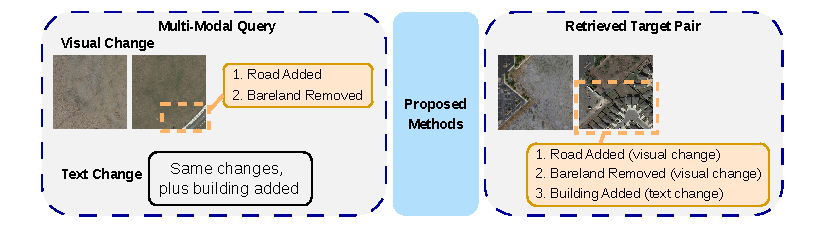
\includegraphics[width=\textwidth]{images/CTCR-RS/figure1-example-eccv.pdf}
    \caption{An example of the Composed Temporal Change
    Retrieval (CTCR-RS) task. Given a reference bi-temporal
    pair depicting two visual changes (Road Added, Bareland
    Removed) and a textual query specifying an additional
    change (Building Added), the system retrieves a target
    pair exhibiting all three changes.}
    \label{fig:chap6_task}
\end{figure}
 
% ============================================================
\section{Related Work}
\label{sec:chap6_rw}
% ============================================================
 
The related work covered in Chapter~\ref{chap:background}
addresses the broader foundations: general VQA and
vision-language architectures, RS image retrieval at the
conceptual level, and CLIP-based cross-modal alignment.
This section focuses on three aspects specific to this
chapter: composed retrieval for single images and video,
bi-temporal change understanding in remote sensing, and
vision-language models adapted for Earth Observation.
 
\subsection{Composed Image and Video Retrieval}
\label{sec:chap6_rw_cir}
 
Composed Image Retrieval (CIR) aims to retrieve a target
image given a visual reference and a textual modifier that
specifies how the target should differ from the
reference~\cite{song2025survey}. Supervised approaches
rely on cross-modal attention, dual-pathway architectures,
or modality fusion mechanisms~\cite{delmas2022artemis,
hosseinzadeh2020composed, huang2024dynamic, wen2024simple}.
To mitigate the scarcity of curated training triplets,
Zero-Shot CIR paradigms map visual concepts into language
token spaces via textual inversion~\cite{baldrati2023zero,
saito2023pic2word}, or caption the reference image using a
pretrained generative VLM and leverage an LLM to recompose
the caption based on the textual modifier~\cite{karthik2023vision}.
More recently, chain-of-thought reasoning has been used
to perform training-free zero-shot
composition~\cite{tang2025reason}.
 
CIR has been successfully adapted to the remote sensing
domain to refine single-image retrieval using textual
queries~\cite{psomas2024cir, wang2024scene, yang2025language}.
However, these methods operate on single-date images and
cannot account for changes occurring across time, motivating
the extension of CIR to the multi-temporal setting.
 
Composed Video Retrieval (CoVR) extends the CIR paradigm to
retrieve target videos based on reference clips and textual
modifiers~\cite{ventura2024covr, ventura2024covr2}. Recent
work explores fine-grained semantic alignment, feature
disentanglement, two-stage training, and pseudo-query
fine-tuning~\cite{gupta2025play, thawakar2024composed,
wu2025fine, zhang2024localizing}. However, CoVR models
continuous actions rather than discrete before/after
satellite states. While the visual structure superficially
resembles a short video (two frames), the semantic nature
of the transition is fundamentally different: bi-temporal
satellite imagery encodes land-use and land-cover change
rather than motion, and the temporal gap between
acquisitions is measured in months or years rather than
video frames. %Adapting CoVR by spatially stacking $I_1$
%and $I_2$ yields poor results on CTCR-RS (0.07 R@1
%zero-shot, 0.11 after fine-tuning), confirming that the
%paradigm transfer fails.
 
\subsection{Bi-Temporal Change Understanding in Remote Sensing}
\label{sec:chap6_rw_change}
 
Bi-temporal change understanding in remote sensing has been
primarily approached through Change Detection (CD) and
Change Captioning (CC). Change detection methods produce
pixel-level binary maps indicating changed versus unchanged
regions~\cite{peng2025deep}, while change captioning methods
generate natural language descriptions of the observed
transitions~\cite{liu2022levir, karaca2025secondcc}.
 
The LEVIR-CC dataset~\cite{liu2022levir} and the SECOND-CC
dataset~\cite{karaca2025secondcc} are the two primary
change captioning resources used in this chapter. LEVIR-CC
consists of bi-temporal aerial image pairs from urban areas
in Texas, USA, each annotated with five independent
human-authored change descriptions. SECOND-CC is a larger
and more diverse change captioning dataset covering a broader
range of urban changes across multiple geographic areas.
Both datasets provide the raw material for the CTCR-RS
pipeline.
 
Cross-modal text-image retrieval has been extended to the
temporal domain by~\cite{hoxha2025selfsupervised},
who propose self-supervised retrieval of time series based
on textual queries. However, this work restricts queries
to one modality only and does not support the composed multi-modal
formulation in which a visual reference pair provides the
base change context. The CTCR-RS task fills this gap by
combining a visual temporal reference with a textual
modifier in a single composed query.
 
\subsection{Vision-Language Models for Earth Observation}
\label{sec:chap6_rw_vlm}
 
Cross-modal retrieval for Earth Observation has undergone
significant progress through the adaptation of large
Vision-Language Models. Early methods bridge the semantic
gap between imagery and language using dual-stream networks
optimized via ranking losses~\cite{cheng2021deep,
yuan2022exploring}. More recently, VLMs such as
RemoteCLIP~\cite{liu2024remoteclip} and
GeoRSCLIP~\cite{zhang2024rs5m} have redefined the
state-of-the-art by leveraging contrastive learning over
massive datasets including RS5M~\cite{zhang2024rs5m},
RSITMD~\cite{RSITMD}, and RSICD~\cite{lu2017exploring}, achieving
robust modality alignment for image-to-text and
text-to-image retrieval.
 

However, existing RS VLMs are pretrained exclusively on
single-date image-text pairs, meaning their embedding spaces
are optimized for static scene description rather than
temporal change representation. While some general-purpose
VLMs can process multiple images as input, they are trained
predominantly on natural images and do not capture the
specific semantics of land-cover change in satellite
imagery. More recently, specialized RS frameworks such as
ChangeChat~\cite{deng2025changechat} and
DeltaVLM~\cite{deng2026deltavlm} have introduced
bi-temporal inputs and change-aware objectives, enabling
interactive change analysis and multi-turn question
answering over bi-temporal pairs. However, none of these
models are designed for the composed retrieval setting, in
which a bi-temporal visual reference and a textual modifier
must be jointly processed to retrieve a target pair
exhibiting the union of both changes. This chapter
introduces two architectures that address this gap:
UniCTCR and StageCTCR.

% ============================================================
\section{The CTCR-RS Task and Dataset}
\label{sec:chap6_dataset}
% ============================================================
 
\subsection{Task Formalization}
\label{sec:chap6_task}
 
Let $\mathcal{I} = (I_1, I_2)$ be a bi-temporal image pair
depicting land-use and land-cover change between two
acquisitions of the same geographic location. We define
$\mathcal{L}(\mathcal{I}) = \{c_1, c_2, \ldots, c_n\}$ as
the set of discrete semantic change labels present in the
pair, where each $c_i$ belongs to a standardized ontology
$\mathcal{O}$ described in
Section~\ref{sec:chap6_ontology}.
 
A CTCR-RS query is defined as a tuple
$(\mathcal{I}_\text{ref}, \mathcal{C}_\text{text})$, where
$\mathcal{I}_\text{ref}$ is a reference bi-temporal image
pair and $\mathcal{C}_\text{text}$ is a textual instruction
specifying additional changes to be composed with the
existing visual changes. The objective is to find a target
pair $\mathcal{I}_\text{tar}$ such that:
\begin{equation}
    \mathcal{L}(\mathcal{I}_\text{tar}) =
    \mathcal{L}(\mathcal{I}_\text{ref}) \cup
    \mathcal{C}_\text{text}
    \quad \text{where} \quad
    \mathcal{L}(\mathcal{I}_\text{ref}) \cap
    \mathcal{C}_\text{text} = \emptyset
\end{equation}
 
Critically, $\mathcal{I}_\text{ref}$ and
$\mathcal{I}_\text{tar}$ depict \textit{different}
geographic locations: the task retrieves archive locations
whose change pattern matches a composed visual-textual query,
analogous to reverse image search over change signatures
rather than tracking changes at a single fixed location over
time. This retrieval task is inherently one-to-many, as
multiple distinct geographic locations will inevitably share
the exact same ground-truth change label set
$\mathcal{L}(\mathcal{I}_\text{tar})$.
 
\subsection{Source Datasets and Domain Scoping}
\label{sec:chap6_sources}
 
The CTCR-RS dataset is constructed from two established
change captioning datasets: LEVIR-CC~\cite{liu2022levir}
and SECOND-CC~\cite{karaca2025secondcc}.
 
\textbf{LEVIR-CC}~\cite{liu2022levir} is a large-scale
remote sensing change captioning dataset built from the
LEVIR-CD change detection benchmark. It consists of 10,077
pairs of bi-temporal aerial images acquired over multiple
urban areas in Texas, USA, at a spatial resolution of
0.5\,m/pixel and a patch size of $256 \times 256$ pixels.
The temporal gap between acquisitions ranges from 5 to 14
years, capturing significant urban development changes.
Each image pair is annotated with five independent
human-authored captions describing the observed changes,
for a total of 50,385 captions. The predominant change
types are building construction and demolition, reflecting
the rapid urban expansion characteristic of the source
region.
 
\textbf{SECOND-CC}~\cite{karaca2025secondcc} is derived
from the SECOND semantic change detection dataset, which
covers six categories of land-cover objects (non-vegetated
ground surface, tree, low vegetation, water, buildings, and
playgrounds) across multiple cities in China. The dataset
contains 6 041 bi-temporal image pairs at $256 \times 256$
pixel resolution, each annotated with five human-authored
change captions, for a total of 30,205 captions. 
 
Both datasets share the key property of providing five
independent human-authored captions per image pair, which
is critical for the robustness of the label extraction
pipeline: redundant descriptions from multiple annotators
allow the LLM to cross-validate change labels and reduce
the impact of individual annotator errors or omissions, as
discussed in Section~\ref{sec:chap6_audit}.
 
 
A third publicly available dataset, RSCC~\cite{chen2025rscc},
covers disaster-related changes including floods,
earthquakes, and wildfires. While the automated curation
pipeline described below is general and could in principle
be applied to RSCC, this dataset covers a fundamentally
different semantic domain from the urban land-cover changes
in LEVIR-CC and SECOND-CC. We intentionally scope this
first benchmark to the urban domain to establish a clean,
controlled evaluation setting with a consistent change
ontology before extending to multi-domain scenarios.
Extending the CTCR-RS pipeline to disaster-related or
rural change datasets is an explicit direction for future
work.
 
\subsection{Caption Synthesis and Label Extraction}
\label{sec:chap6_extraction}
 
The first challenge in constructing CTCR-RS is transforming
the five heterogeneous, free-form human captions associated
with each image pair into a consistent set of structured
change labels. We employ Gemma~3~\cite{gemma2025} as a
semantic mapper, using a Chain-of-Thought (CoT) prompting
strategy to simultaneously synthesize redundant descriptions
and extract a normalized set of change labels.
 
The extraction proceeds in six reasoning steps: (1) object
analysis: listing all objects mentioned across the five
captions; (2) change type analysis: identifying all types
of changes described; (3) unique information extraction:
merging paraphrases and removing redundancy; (4) spatial
analysis: identifying where changes occur within the
image; (5) synthesis: combining the most important
elements into a single concise caption; (6) normalization, outputting a JSON array of object-change pairs. The full
prompt used for this stage is as follows:
 
\begin{quote}
\small
\textbf{System:} You are an expert in analyzing satellite
image changes using systematic reasoning.
 
\textbf{User:} Analyze the following 5 captions describing
a satellite image change for \{filename\}:
\{captions\_text\}
 
Follow these steps to reason through the changes:
 
STEP 1 -- OBJECT ANALYSIS: List all objects mentioned.
 
STEP 2 -- CHANGE TYPE ANALYSIS: List all types of changes.
 
STEP 3 -- UNIQUE INFORMATION EXTRACTION: Merge paraphrases,
remove redundancy, and list all distinct pieces of
information.
 
STEP 4 -- SPATIAL ANALYSIS: Where do changes occur?
 
STEP 5 -- SYNTHESIS: Combine the most important elements
into one concise caption.
 
STEP 6 -- NORMALIZED CHANGES: From the above, output a
JSON array of object-change pairs.
 
\textbf{Rules:}
\begin{itemize}
    \item Use common sense to normalize object names to a
    standard form (e.g., ``gray structures'' $\to$
    ``building'', ``soil area'' $\to$ ``bareland'').
    \item Use common sense to normalize change types (e.g.,
    ``constructed'' $\to$ ``added'', ``demolished'' $\to$
    ``removed'').
    \item If the change involves replacing one class with
    another (e.g., bareland with vegetation), treat it as
    two operations: \{object: ``bareland'', change:
    ``removed''\} and \{object: ``vegetation'', change:
    ``added''\}.
    \item For ``X replaced Y'' or ``X replaces Y'': output
    \{object: Y, change: ``removed''\} and \{object: X,
    change: ``added''\}.
    \item For "X is replaced by Y": output {object: X, change: "removed"} 
  and {object: Y, change: "added"}.
\item Never output objects with "no change" — omit unchanged objects 
entirely.
\item Ignore location words and process words.
\item Only include pairs explicitly stated in the captions.
\end{itemize}
\textbf{Final Optimal Caption}:
One mid-sized caption around 25 words summarizing the main scene 
differences, not listing every single change

\textbf{Normalized Changes}:
JSON array of {"object": "...", "change": "..."}
\end{quote}
 
A critical design choice in this stage is the decomposition
of inter-class transitions. For changes involving a semantic
class transition (e.g., a forest cleared for an excavation
site), the model is instructed to decompose the event into
two independent operations: Removal, representing the
disappearance of the initial state, and Addition,
representing the appearance of the final state. This ensures
that the resulting change sets correctly capture both sides
of a transition, supporting compositional matching in
retrieval.
 
\subsection{Taxonomy and Change Ontology}
\label{sec:chap6_ontology}
 
The initial extraction pass produces normalized but still
potentially inconsistent labels. A second pass with
Gemma~3 enforces a controlled vocabulary of 14
standardized geospatial change types, defined over six
broad change categories and three change types:
 
\textbf{Change categories:} Building, Bareland, Water,
Vehicle, Vegetation, Road.
 
\textbf{Change types:} Added, Removed, Replaced (the latter
specifically accounts for intra-class transitions such as
infrastructure upgrades or building redevelopments).
 
This yields $6 \times 3 = 18$ theoretical combinations,
reduced to 14 in practice as Replaced is only meaningful
for infrastructure classes (Building, Road). Fine-grained
object descriptors are consolidated into these broad
macroscopic categories (e.g., ``villa'', ``apartment'', and
``factory'' all map to Building), while action verbs are
normalized to the three allowed change types (e.g.,
``constructed'', ``erected'', ``built'' all map to Added).
 The full prompt used for this normalization stage is as
follows:
 
\begin{quote}
\small
\textbf{System:} You are an expert in satellite image change
analysis.
 
\textbf{User:} Here are captions and their current
normalized\_changes for multiple entries:
\{batch\_json\}
 
Your task: review and correct ONLY the
``normalized\_changes'' field for each entry.
 
\textbf{Ontology:}
\begin{itemize}
    \item Broad types: building, vegetation, road, water,
    vehicle, bareland.
    \item Subtypes: any descriptive term is allowed.
    \item Allowed change values: added, removed, replaced.
\end{itemize}
 
\textbf{Rules:}
\begin{enumerate}
    \item Verify that all changes are consistent with
    captions.
    \item Correct mislabeled objects to match the ontology.
    \item Merge duplicate changes (same broad type + same
    change type).
    \item Normalize all free-text change values into the
    allowed set above.
    \item Drop any single change with ``no\_change''.
    \item Output must be valid JSON only.
\end{enumerate}
\end{quote}

\begin{figure}[ht]
    \centering
    % NOTE: insert Figure 2 from the main paper here
    % (full dataset curation pipeline figure)
    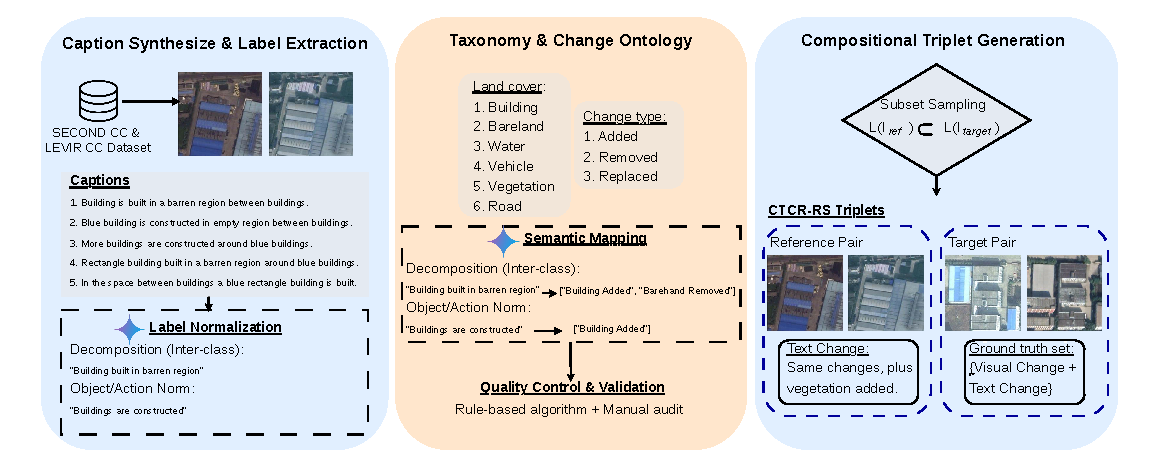
\includegraphics[width=\textwidth]{images/CTCR-RS/figure2-dscuration-eccv.pdf}
    \caption{The CTCR-RS dataset curation pipeline from raw
    captions to composed retrieval triplets. Raw captions
    from LEVIR-CC and SECOND-CC are processed through
    caption synthesis and label extraction (Stage~1),
    taxonomy normalization (Stage~2), quality control, and
    compositional triplet generation.}
    \label{fig:chap6_pipeline}
\end{figure}
 
\subsection{Dataset Statistics and Characteristics}
\label{sec:chap6_stats}
 
The CTCR-RS dataset comprises 30,179 unique compositional
triplets. Figure~\ref{fig:chap6_stats} summarizes the key
distributional properties.
 
\begin{figure}[ht]
    \centering
    % NOTE: insert Figure 3 from the main paper here
    % (three-panel statistics figure: global change frequency
    % visual vs text, co-occurrence heatmap, distribution of
    % number of changes per triplet component)
    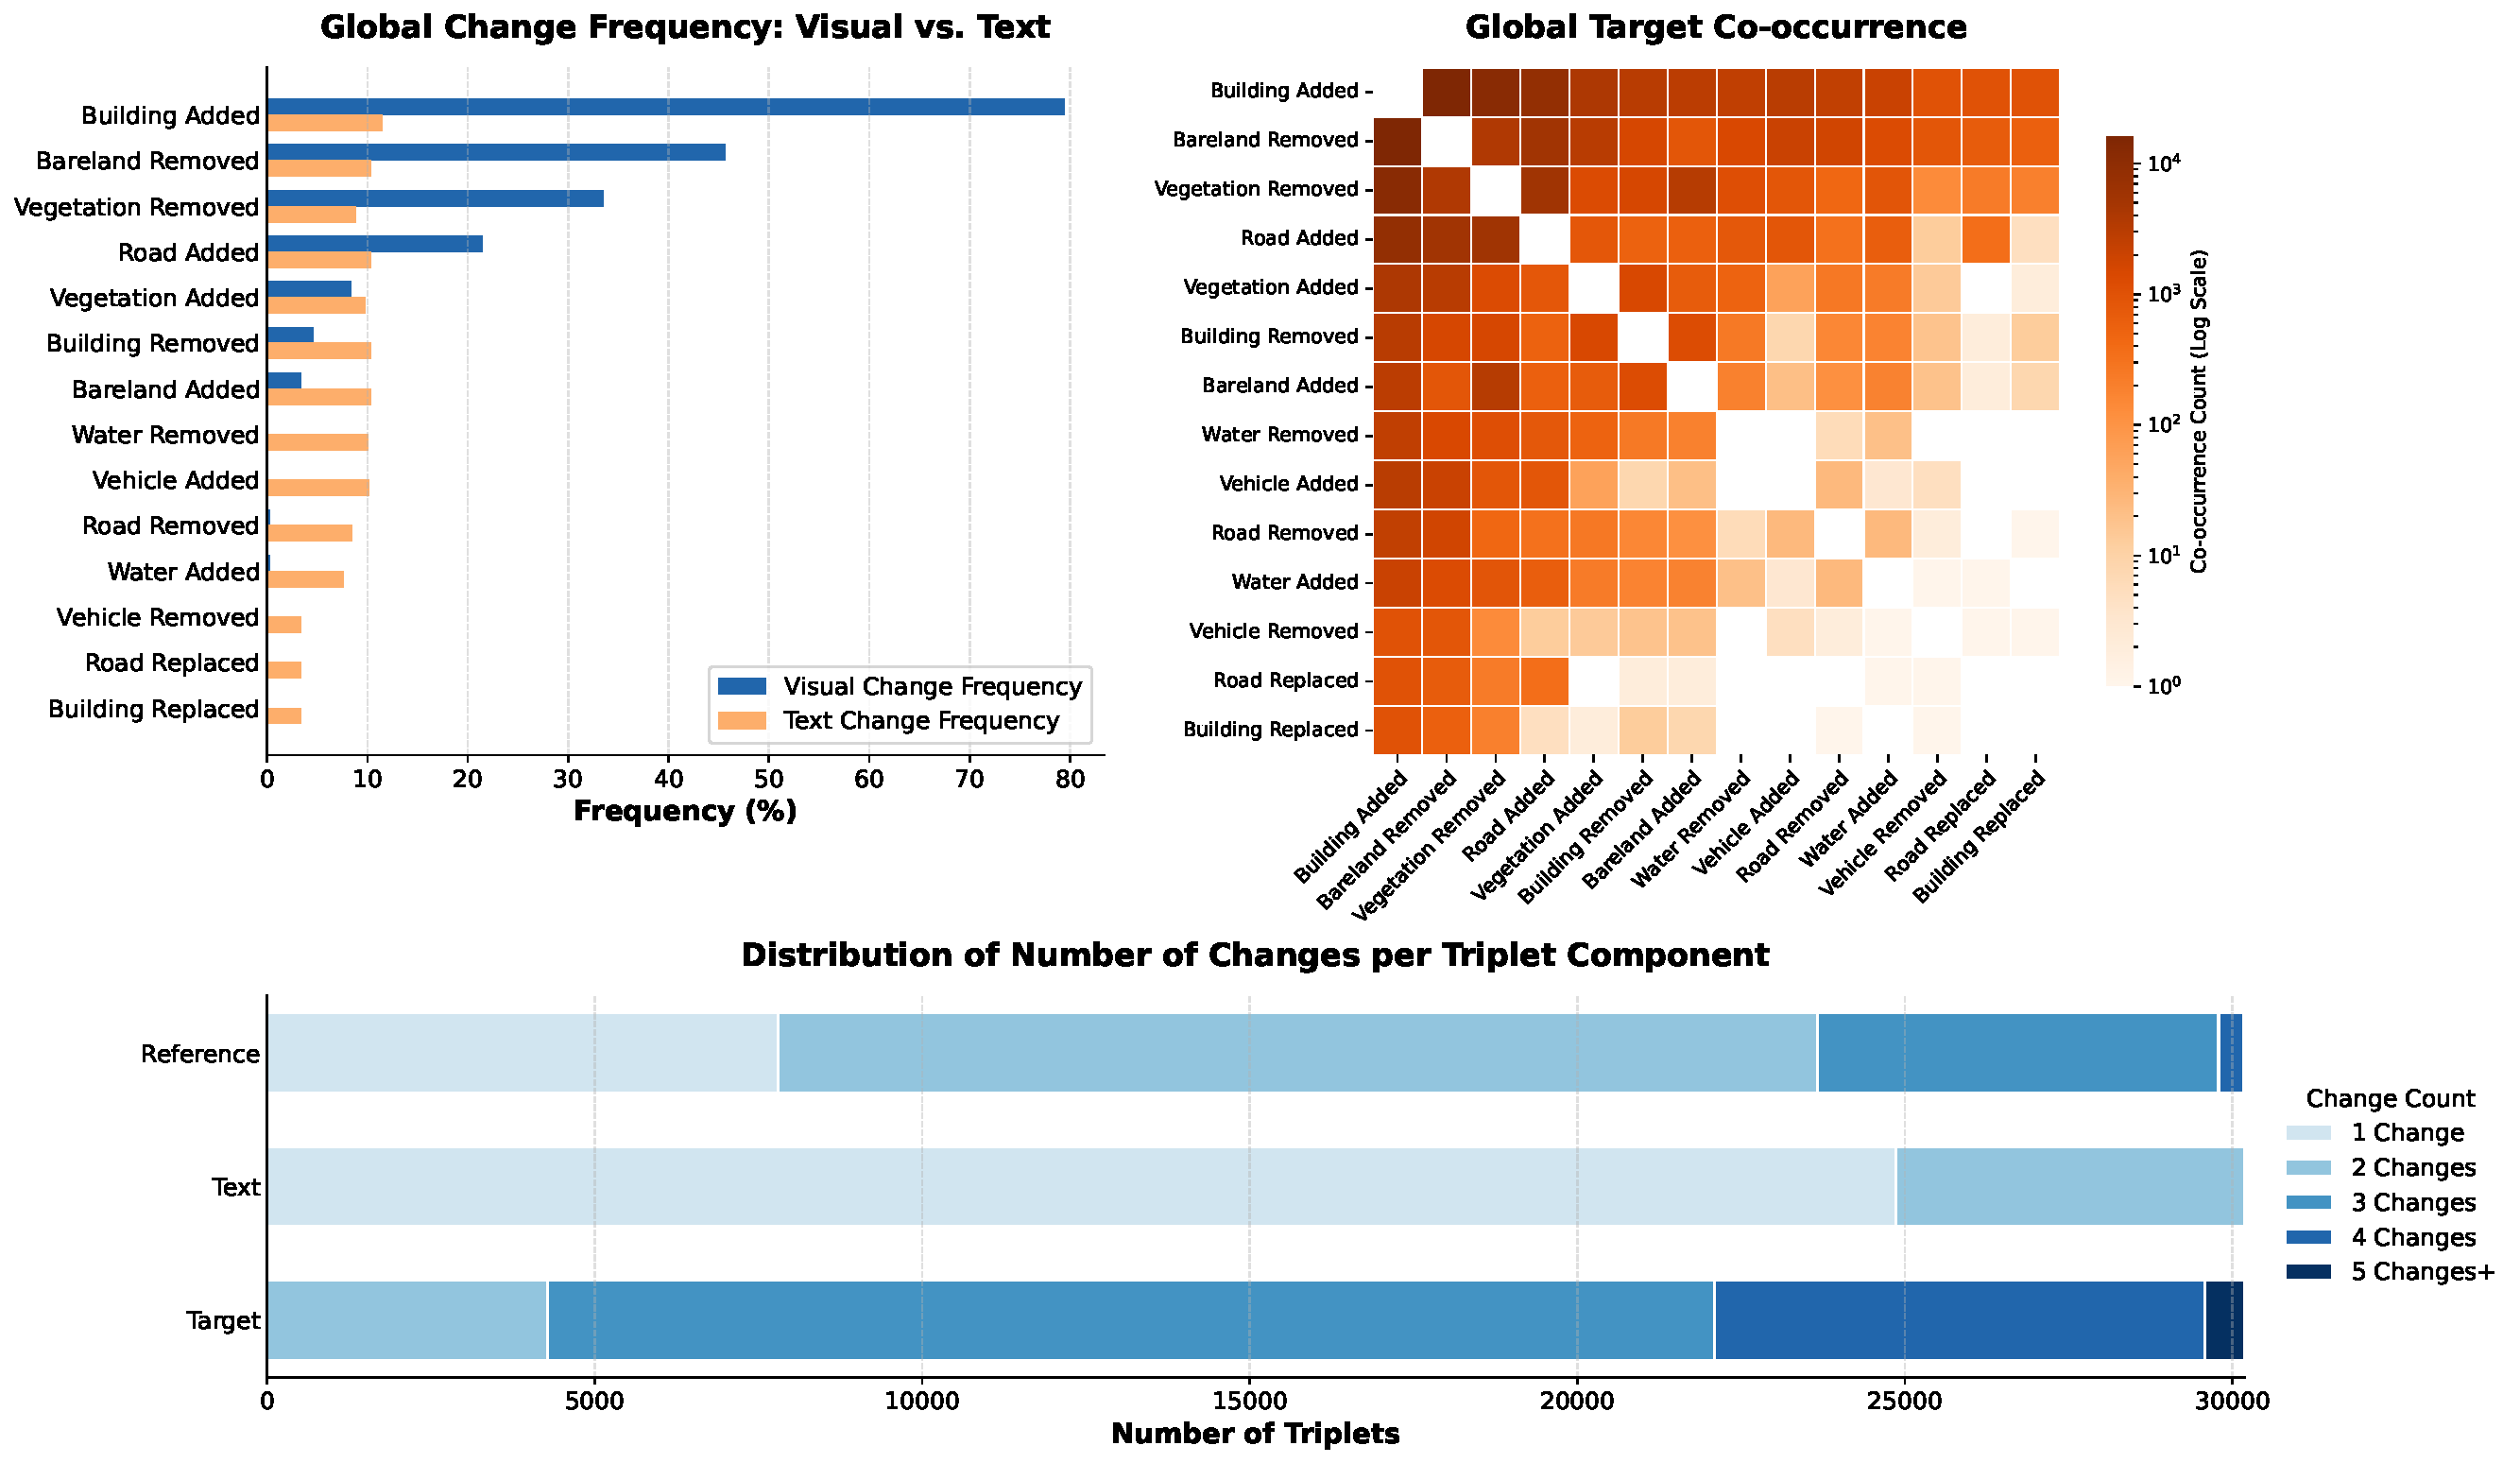
\includegraphics[width=\textwidth]{images/CTCR-RS/master_dataset_figure.pdf}
    \caption{CTCR-RS dataset statistics. \textbf{Top left}:
    visual (blue) vs.\ text (orange) change frequencies,
    demonstrating balanced text queries despite heavily
    unbalanced visual changes. \textbf{Top right}:
    log-scaled co-occurrence heatmap highlighting change
    correlations. \textbf{Bottom}: change counts per triplet
    component, visualizing the subset-superset task
    formulation.}
    \label{fig:chap6_stats}
\end{figure}
 
\textbf{Change frequency and bias mitigation.} The visual
change distribution $\mathcal{L}(\mathcal{I}_\text{ref})$
exhibits  a natural long-tail characteristic reflecting the
urban expansion dynamic dominant in LEVIR-CC and SECOND-CC:
Building Added and Bareland Removed
collectively dominate, while Replaced categories remain
rare, reflecting the infrequency of intra-class transitions
in the source datasets. To prevent the model from overfitting
to these visual changes, the text change synthesis ensures a
more balanced distribution of text queries
$\mathcal{C}_\text{text}$: less common change types are
more frequently selected as the textual modifier, resulting
in the orange distribution shown in
Figure~\ref{fig:chap6_stats} (top left).
 
\textbf{Change co-occurrence.} Building Added and Bareland
Removed co-occur strongly (Figure~\ref{fig:chap6_stats},
top right), reflecting the predominant urban expansion
pattern in the source datasets: new construction typically
occurs on previously bare land. This strong co-occurrence
is important to keep in mind when interpreting retrieval
performance: models that learn this correlation can partially
exploit it as a shortcut rather than performing genuine
compositional retrieval.
 
\textbf{Compositional complexity.} CTCR-RS moves beyond
single-attribute modifications. On average, each target
pair contains 3.2 simultaneous semantic changes. Notably,
over 85.81\% of the triplets require the model to compose
across three or more concurrent changes, a level of
complexity that challenges all baseline architectures as
shown in Section~\ref{sec:chap6_experiments}.
 
\textbf{One-to-many mapping.} Unlike standard CIR, the
CTCR-RS task is inherently one-to-many: multiple distinct
geographic locations can undergo identical land-use and
land-cover transitions. During training, the model
encounters an average of 39.1 positive targets per unique
change composition, a density that increases to 79.3 in the
test set, where 9,275 samples concentrate across only 117
unique compositions (compared to 298 in training). This
property has two important implications. First, it motivates
the Multiple Positives Enhanced NCE Loss described in
Section~\ref{sec:chap6_unictr_training}, which encourages
the model to learn generalized land-cover transition
representations rather than memorizing specific image
instances. Second, it means that standard retrieval metrics
computed against a single positive underestimate true
performance; the evaluation protocol described in
Section~\ref{sec:chap6_setup} accounts for all valid
positives.
 
\subsection{Compositional Triplet Generation}
\label{sec:chap6_triplets}
 
Retrieval triplets are constructed by exploiting the
subset-superset relationship between change label sets.
For every image pair $\mathcal{I}_\text{tar}$, we search
for potential reference pairs $\mathcal{I}_\text{ref}$
such that $\mathcal{L}(\mathcal{I}_\text{ref}) \subset
\mathcal{L}(\mathcal{I}_\text{tar})$. To ensure manageable
complexity while maintaining diversity, we restrict the
number of additional text changes
$n = |\mathcal{L}(\mathcal{I}_\text{tar}) \setminus
\mathcal{L}(\mathcal{I}_\text{ref})|$ to $n \in \{1, 2\}$.
 
Rather than using raw, inconsistent human captions as the
textual modifier, we generate the textual query
$\mathcal{C}_\text{text}$ using a standardized template:
\textit{``I want the same changes as in the reference pair,
plus [Extra Label(s)]''}. This ensures annotation precision
and consistency across the dataset, at the cost of
constraining the query to templated natural language rather
than free-form instructions, a limitation acknowledged
in Section~\ref{sec:chap6_conclusion}.
See Figure~\ref{fig:chap6_pipeline} for a visual overview of
the full dataset curation pipeline.

\subsection{Human Audit and Quality Validation}
\label{sec:chap6_audit}
 
To ensure the fidelity of the extracted change labels, we
conduct a rigorous manual audit on 600 stratified samples
randomly drawn from the dataset. For each sample, an expert
auditor compares the five raw human-authored captions, the
final normalized label set extracted by the LLM, and the
actual visual changes visible in the bi-temporal images.
 
\textbf{Overall results.} The LLM achieves an overall
extraction accuracy of 83.5\%, successfully and completely
mapping the free-form text to the correct visual reality in
501 of the 600 samples. Of the 99 failure cases (16.5\%),
78 errors (13.0\%) are true LLM hallucinations or extraction
misses where the model fails to properly synthesize the
captions, and 21 errors (3.5\%) stem from omissions or
errors in the original change captions themselves.
 
We provide examples of each outcome: LLM extraction
successes (Figure~\ref{fig:chap6_audit_success}), LLM
extraction misses (Figure~\ref{fig:chap6_audit_miss}),
and annotator errors and ambiguities
(Figure~\ref{fig:chap6_audit_error}).
 
\begin{figure}[ht]
    \centering
    % NOTE: insert Figure 1 from the supplementary here
    % (audit successes: two examples from LEVIR and SECOND
    % showing correct LLM extraction)
    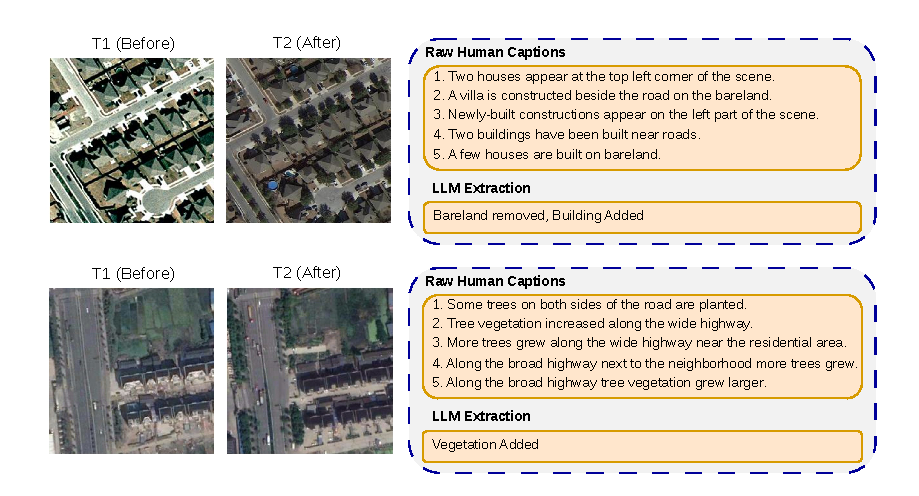
\includegraphics[width=0.85\textwidth]{images/CTCR-RS/supp-figure1-3.pdf}
    \caption{Audit successes: examples of correct LLM
    extraction across both source datasets. \textbf{Top
    (LEVIR-CC)}: the LLM correctly normalizes a building
    construction on bareland as Building Added + Bareland
    Removed. \textbf{Bottom (SECOND-CC)}: the LLM captures
    the distinct changes described by the annotators and maps
    them to the standard ontology.}
    \label{fig:chap6_audit_success}
\end{figure}
 
\begin{figure}[ht]
    \centering
    % NOTE: insert Figure 2 from the supplementary here
    % (LLM extraction misses: two examples where LLM
    % missed an explicitly stated label)
    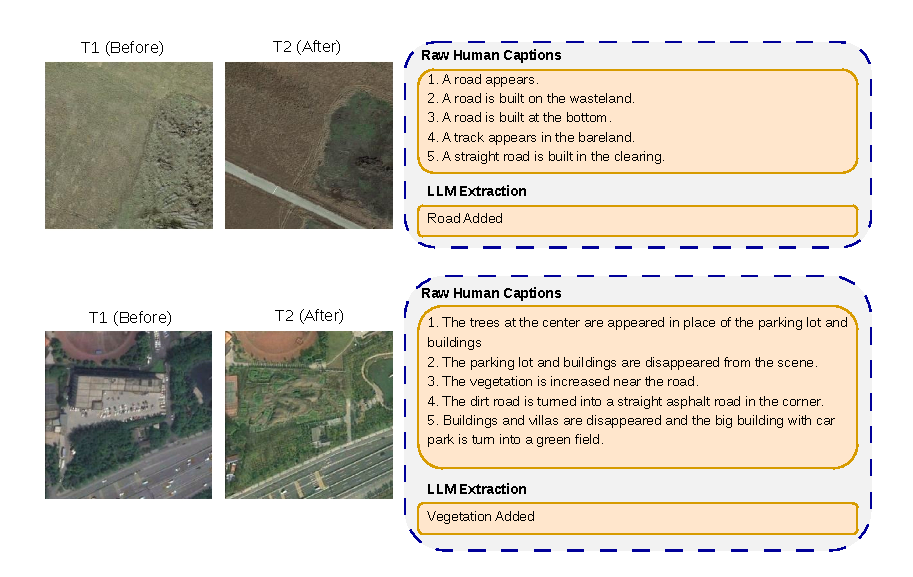
\includegraphics[width=0.85\textwidth]{images/CTCR-RS/supp_figure2.pdf}
    \caption{LLM extraction misses: examples where the
    pipeline failed to capture explicitly stated information.
    \textbf{Top (LEVIR-CC)}: Road Added is extracted but
    Bareland Removed is missed despite annotators mentioning
    the road was built on wasteland. \textbf{Bottom
    (SECOND-CC)}: Vegetation Added is extracted but Building
    Removed is dropped.}
    \label{fig:chap6_audit_miss}
\end{figure}
 
\begin{figure}[ht]
    \centering
    % NOTE: insert Figure 3 from the supplementary here
    % (annotator errors/ambiguity: temporal reversal, annotator
    % contradiction)
    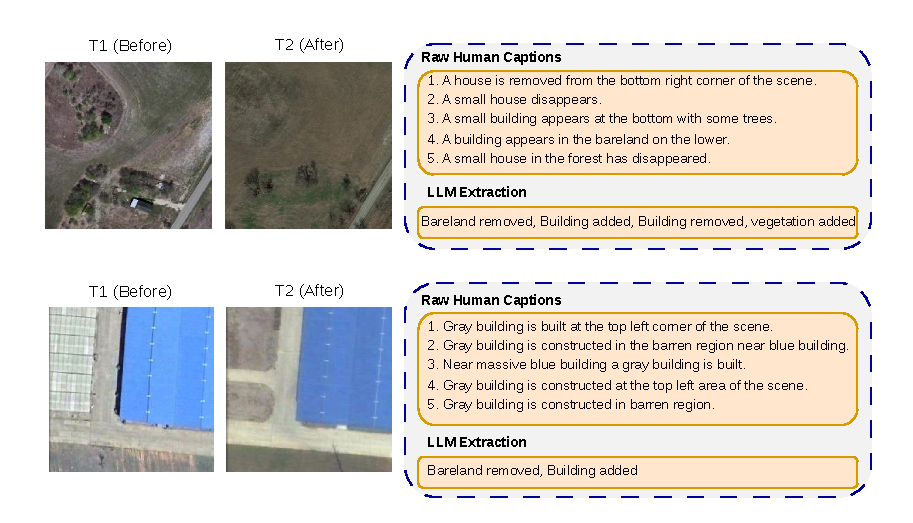
\includegraphics[width=0.85\textwidth]{images/CTCR-RS/supp-figure3.pdf}
    \caption{Errors originating from the original captions
    rather than the LLM pipeline. \textbf{Top (LEVIR-CC)}:
    annotator contradiction: some annotators describe a
    building as removed while others say it appears; the LLM
    extracts both. \textbf{Bottom (SECOND-CC)}: temporal
    reversal: the images show a demolition but the
    annotators describe it as construction.}
    \label{fig:chap6_audit_error}
\end{figure}
 
\textbf{LLM extraction misses (13.0\%).} These errors occur
when the model fails to capture all explicitly stated changes
from the captions. A common pattern is the omission of the
complementary removal label when annotators describe a
replacement (e.g., extracting Road Added but missing
Bareland Removed despite the annotators specifying the road
was built on wasteland). These errors are non-systematic and
do not concentrate on specific change types, suggesting they
are caused by the inherent difficulty of multi-label
extraction from ambiguous natural language rather than
systematic biases in the pipeline.
 
\textbf{Annotator errors and ambiguity (3.5\%).} A
qualitatively distinct error category arises not from the
LLM but from the source annotations themselves. Two
recurring patterns are particularly notable. First,
annotator contradiction: for the same bi-temporal pair,
some annotators describe a building as being demolished
while others describe a new building appearing, possibly
due to difficulty interpreting the temporal ordering of
before/after images. The LLM, faced with contradictory
instructions, extracts both changes. Second, temporal
reversal: annotators chronologically reverse the event,
describing a demolition as construction or vice versa. These errors
validate that 3.5\% of failures reflect genuine annotation
difficulty in the source datasets rather than deficiencies
in the curation pipeline.
 
\subsection{Dataset Splitting}
\label{sec:chap6_split}
 
The dataset is partitioned at the bi-temporal image pair
level \textit{prior} to triplet construction, yielding
11,660 / 9,244 / 9,275 triplets for training, validation,
and testing, corresponding to 3,768 / 925 / 945 unique
target image pairs respectively. Splitting at the image pair
level ensures that no bi-temporal image pair appears in
multiple splits, preventing information leakage through
shared visual content between training and evaluation
triplets.
 
% ============================================================
\section{Methodology}
\label{sec:chap6_method}
% ============================================================
 
To address the CTCR-RS task, we propose two complementary
architectures that progressively move from end-to-end latent
fusion to explicit semantic decomposition.
Figure~\ref{fig:chap6_arch} provides an overview of both.
 
\begin{figure}[ht]
    \centering
    % NOTE: insert Figure 4 from the main paper here
    % (architectural overview: UniCTCR left, StageCTCR right)
    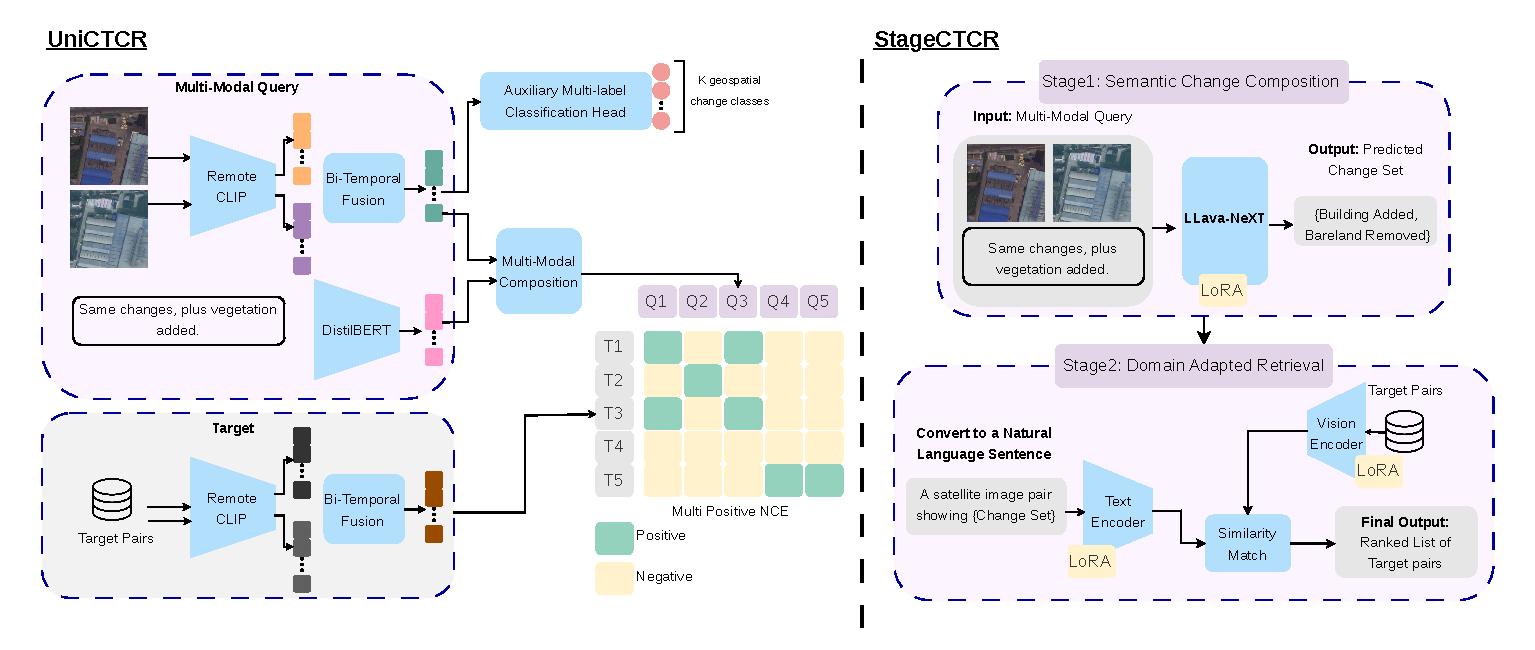
\includegraphics[width=0.85\textwidth]{images/CTCR-RS/figure-architecture-eccv.pdf}
    \caption{Architectural overview. \textbf{Left}: UniCTCR
    performs implicit multi-modal composition via bi-temporal
    feature fusion and Multi Positive NCE training.
    \textbf{Right}: StageCTCR decouples the task into
    VLM-based semantic composition (Stage~1, LLaVA-NeXT)
    and domain-adapted retrieval (Stage~2, RSICD-CLIP).}
    \label{fig:chap6_arch}
\end{figure}
 
\subsection{UniCTCR}
\label{sec:chap6_unictr}
 
UniCTCR is an end-to-end architecture that learns a joint
multi-modal change representation through dedicated fusion
and composition modules.
 
\subsubsection{Feature Extraction}
\label{sec:chap6_unictr_features}
 
Given a reference image pair $\mathcal{I} = (I_1, I_2)$
and a query text $\mathcal{C}_\text{text}$, we extract
unimodal representations as follows.
 
\textbf{Visual features.} For each image in the pair, we
use a pretrained RemoteCLIP~\cite{liu2024remoteclip} model
(ViT-B/32 backbone) to extract global embeddings $v_1,
v_2 \in \mathbb{R}^d$. RemoteCLIP is pretrained via
contrastive learning on large-scale RS image-text pairs,
providing representations that encode both fine-grained
spatial detail and high-level semantic content relevant to
land-cover categories.
 
\textbf{Textual features.} The query text
$\mathcal{C}_\text{text}$ is processed using pretrained
DistilBERT~\cite{sanh2019distilbert}, projecting the
\texttt{[CLS]} token to the joint embedding dimension $d$
to obtain the text representation $t \in \mathbb{R}^d$.
 
Both encoders are linearly projected into a shared $d = 512$
dimensional space and kept frozen during training, with all
trainable parameters concentrated in the fusion and
composition modules described below.
 
\subsubsection{Bi-Temporal Fusion}
\label{sec:chap6_unictr_fusion}
 
To aggregate the temporal information from $(v_1, v_2)$
into a unified semantic change representation
$v_\text{change}$, we evaluate three fusion strategies:
 
\textbf{Subtraction.} The most direct temporal modeling:
$v_\text{change} = v_2 - v_1$. This operation encodes the
direction of change in the embedding space, but assumes
that the difference vector is semantically meaningful, which
may not hold for complex multi-class transitions.
 
\textbf{Concatenation.} A learned linear projection of the
concatenated temporal features $[v_1; v_2]$. This allows
the model to learn a non-linear mapping from the joint
representation to a change embedding, without imposing the
strong assumption of the subtraction approach.
 
\textbf{Cross-Attention.} A bidirectional attention
mechanism over the $7 \times 7$ spatial patch embeddings
from both timesteps. Features are processed through a
3-layer transformer block (16 heads), mean-pooled, and
projected via a two-layer MLP, capturing complex
spatio-temporal interactions at the patch level. While
computationally more expensive, this approach can in
principle identify which spatial regions changed and reason
about the nature of the change, rather than operating on
global embeddings alone.
 
%Our ablation study (Table~\ref{tab:chap6_fusion}) shows
%that Concatenation achieves the highest global performance,
%marginally outperforming Subtraction and Cross-Attention.
%The narrow spread between the three strategies (less than
%4\% relative difference) suggests that the temporal fusion
%strategy is less critical than the downstream composition
%quality, which is the dominant bottleneck in this task.
 
\subsubsection{Multi-Modal Composition}
\label{sec:chap6_unictr_composition}
 
To fuse $v_\text{change}$ with the textual modification
$t$, we concatenate them into a joint representation
$h_\text{joint} = [v_\text{change}; t]$ and evaluate two
composition heads:
 
\textbf{MLP.} A standard two-layer MLP with ReLU
activation and dropout applied to $h_\text{joint}$ to
produce the final retrieval embedding $e_\text{ret}$.
 
\textbf{Gated Residual.} A dynamic pathway that modulates
the visual change based on the textual instruction. A
modulation gate $g$ (tanh activation) and a residual
correction $r$ are computed via parallel MLPs:
\begin{equation}
    e_\text{ret} = \text{Normalize}(v_\text{change}
    \odot g + r)
\end{equation}
This allows the model to selectively emphasize or suppress
aspects of the visual change representation based on what
the textual query requests.
%Despite its conceptual appeal,
%the standard MLP head substantially outperforms the Gated
%Residual in practice (0.23 vs. 0.12 R@1), suggesting that
%the dynamic modulation is harder to train with the
%available data.
 
\subsubsection{Target Encoding and Auxiliary Objective}
\label{sec:chap6_unictr_target}
 
Candidate target pairs $(I_1', I_2')$ in the retrieval
database are processed through the identical RemoteCLIP
encoder and bi-temporal fusion module to yield
$e_\text{target}$, enabling standard cosine similarity
matching against $e_\text{ret}$.
 
An auxiliary multi-label classification head is applied
directly to $v_\text{change}$ to predict the presence of
the $K$ land-cover change classes within the reference
pair. This two-layer MLP is trained with binary
cross-entropy and serves as an explicit regularizer: it
forces the bi-temporal fusion module to produce
semantically meaningful change representations before the
composition module operates on them.
 
\subsubsection{Training Objectives}
\label{sec:chap6_unictr_training}
 
To address the one-to-many mapping property of the
CTCR-RS task, UniCTCR is trained with a composite
objective. Let $\mathcal{P}(i)$ be the set of all valid
positive targets for query $i$, and $S_{ij} =
(e_\text{ret}^{(i)} \cdot e_\text{target}^{(j)}) / \tau$
be the scaled cosine similarity with temperature $\tau$.
The Multiple Positives Enhanced NCE loss aggregates
probability mass over all valid positives:
\begin{equation}
    \mathcal{L}_\text{nce}^{(i)} = -\log
    \frac{\sum_{p \in \mathcal{P}(i)} \exp(S_{ip})}
    {\sum_{j \in \mathcal{A}(i)} \exp(S_{ij})}
    \label{eq:mpnce}
\end{equation}
where $\mathcal{A}(i)$ represents all samples in the
batch. This is coupled with a similarity regularization
term $\mathcal{L}_\text{sim}^{(i)}$ that directly maximizes
the mean unscaled cosine similarity of all positive pairs.
The full training objective is:
\begin{equation}
    \mathcal{L}_\text{total} = \frac{1}{N}
    \sum_{i=1}^N \left(
    \mathcal{L}_\text{nce}^{(i)} +
    \alpha \mathcal{L}_\text{sim}^{(i)}
    \right) + \lambda \mathcal{L}_\text{aux}
    \label{eq:unictr_loss}
\end{equation}
UniCTCR is trained with AdamW, learning rate $5 \times
10^{-4}$, weight decay 0.01, batch size 512, dropout 0.2,
for 40 epochs.
 
\subsection{StageCTCR}
\label{sec:chap6_stagectcr}
 
Motivated by the oracle analysis of UniCTCR (see Table \ref{tab:chap6_fusion}), which reveals
that the primary bottleneck lies in multi-modal composition
rather than retrieval, StageCTCR explicitly decomposes the
problem into two independent stages: semantic change
composition followed by domain-adapted retrieval. This
eliminates the need for learned latent fusion, replacing it
with the explicit reasoning capabilities of a pretrained
VLM.
 
\subsubsection{Stage 1: Semantic Change Composition}
\label{sec:chap6_stage1}
 
The first stage employs LLaVA-NeXT~\cite{liu2024llavanext}
as a semantic change composition engine. Given the textual
query structure ``\textit{I want the same changes as the
reference pair, plus $\mathcal{C}_\text{text}$}'', the VLM
must visually deduce the changes present in
$\mathcal{I}_\text{ref}$ and integrate them with
$\mathcal{C}_\text{text}$ to predict the full target change
set $\mathcal{L}(\mathcal{I}_\text{tar})$.
 
To provide the VLM with a single image input, the reference
pair is spatially concatenated into a unified composite
image $I_\text{comp} \in \mathbb{R}^{H \times 2W \times 3}$,
with ``BEFORE'' and ``AFTER'' text markers digitally
overlaid to provide explicit temporal grounding. LLaVA-NeXT
is fine-tuned via LoRA to output a strict, comma-separated
string from the change ontology.
 
LoRA is applied to all linear layers within the language
model backbone (attention and feed-forward projections),
while the vision tower, multimodal projector, and language
modeling head are kept frozen. Configuration: rank $r = 64$,
scaling factor $\alpha = 128$, dropout 0.05, fine-tuned for
3 epochs at learning rate $2 \times 10^{-4}$ with
AdamW~\cite{adamw}.
 
\subsubsection{Stage 2: Domain-Adapted Retrieval}
\label{sec:chap6_stage2}
 
The second stage is a dedicated retrieval backbone. A CLIP
model pretrained on RSICD~\cite{lu2017exploring} is
fine-tuned via LoRA to project both modalities into a
shared retrieval space. The structured target list
$\mathcal{L}(\mathcal{I}_\text{tar})$ predicted by Stage~1
is converted into a natural language prompt (e.g., ``\textit{A
satellite image pair showing [change list]}''), which the
CLIP text encoder processes to yield the text embedding
$e_\text{text} \in \mathbb{R}^d$. Symmetrically, candidate
target pairs are horizontally concatenated,
letterbox-padded to $224 \times 224$, and processed by the
CLIP vision encoder to yield $e_\text{target} \in
\mathbb{R}^d$.
 
LoRA is applied to the projection layers of both CLIP
encoders (configuration: $r = 16$, $\alpha = 32$, dropout
0.05), and both encoders are fine-tuned jointly using a
symmetric InfoNCE loss for 5 epochs at learning rate
$10^{-4}$ with AdamW.
 
% ============================================================
\section{Experimental Study}
\label{sec:chap6_experiments}
% ============================================================
 
\subsection{Experimental Setup}
\label{sec:chap6_setup}
 
\textbf{Evaluation metrics.} We report standard retrieval
metrics: Recall at $k$ (R@1, R@5, R@10, R@20), Median
Rank (MedR, lower is better), and Mean Average Precision
at 5 (mAP@5). All metrics are computed over the full test
set. Since the task is one-to-many, a retrieved pair is
considered correct if it belongs to the set of all valid
positives for the query composition.
 
\textbf{Complexity stratification.} In addition to the
global test set, results are reported across two orthogonal
complexity dimensions. \textit{Text Query complexity} refers
to the number of additional changes specified in
$\mathcal{C}_\text{text}$ (1 or 2). \textit{Visual Query
complexity} refers to the number of changes present in the
reference image pair $\mathcal{I}_\text{ref}$ (1, 2, or
$>$2). The two stratifications are overlapping and not
mutually exclusive, allowing independent assessment of
textual composition difficulty versus visual change
disentanglement difficulty.
 
\textbf{Oracle baselines.} Two oracle baselines establish
upper bounds. The \textit{Text-Only Oracle} for UniCTCR
replaces the composed query with the full ground-truth
target description, measuring the upper bound of
text-to-visual retrieval within the UniCTCR architecture.
The \textit{GT+CLIP Upper Bound} applies the same oracle
strategy within StageCTCR's retrieval stage, replacing
LLaVA-NeXT predictions with ground-truth labels. Neither
oracle is a realistic inference-time setting; both serve
to isolate retrieval difficulty from composition difficulty.
 
\textbf{Baselines.} We compare against SEARLE~\cite{baldrati2023zero}
(zero-shot CIR using only the post-change image $I_2$) and
CoVR~\cite{ventura2024covr} (composed video retrieval,
adapted by stacking $I_1$ and $I_2$ spatially),
zero-shot and after fine-tuning on CTCR-RS.
 
\subsection{UniCTCR: Ablation of Fusion Strategies and
Composition Heads}
\label{sec:chap6_unictr_results}
\textbf{Fusion strategy.} Concatenation achieves the
highest global performance (R@1 = 0.24, mAP@5 = 0.66),
marginally outperforming Subtraction (0.23 R@1) and
Cross-Attention (0.22 R@1). The narrow spread between the
three strategies (approximately 4\% relative difference)
suggests that the temporal fusion strategy is less critical
than the downstream composition quality. Cross-Attention
provides better results at high visual complexity ($>$2
changes), likely because patch-level spatial attention
helps disentangle overlapping changes, but Concatenation
is more robust across the majority of the dataset. This
indicates that simpler fusion adequately captures
multi-modal relationships for global feature-level
operations.
 
\textbf{Composition head.} The standard MLP head
substantially outperforms the Gated Residual fusion
(0.23 vs. 0.12 R@1 globally), with the Gated Residual
struggling particularly on simpler single-change queries
where its dynamic gating mechanism appears to overfit.
 
\textbf{Oracle analysis.} The Text-Only Oracle achieves
R@1 = 0.30, exceeding the best UniCTCR configuration.
This establishes an important reference point: the
performance gap between UniCTCR (0.24) and the oracle
(0.30) is attributable entirely to the composition step,
confirming that identifying and fusing the composed
visual-textual change is the primary bottleneck. The
oracle also underperforms on top-rank metrics for single
visual changes (0.31 vs. 0.42 R@1), where the visual
reference provides stronger signal than a text description.
 
\begin{table}[htb]
\centering
\footnotesize
\caption{Ablation of bi-temporal fusion strategies and
composition heads for UniCTCR. \textbf{Global} reports
results on the full test set; subsequent rows stratify by
text and visual complexity. Best non-oracle R@1 result per
complexity level in \textbf{bold}.}
\label{tab:chap6_fusion}
\resizebox{0.85 \textwidth}{!}{
\begin{tabularx}{\textwidth}{ll
    >{\centering\arraybackslash}X
    >{\centering\arraybackslash}X
    >{\centering\arraybackslash}X
    >{\centering\arraybackslash}X
    >{\centering\arraybackslash}X
    >{\centering\arraybackslash}X}

\toprule
\textbf{Method} & \textbf{Complexity}
& R@1 & R@5 & R@10 & R@20 & MedR$\downarrow$ & mAP@5 \\
\midrule
\multirow{6}{*}{MLP + Concat.}
& Global           & \textbf{0.24} & 0.47 & 0.62 & 0.72 & 6  & 0.66 \\
& 1 Text Change    & \textbf{0.22} & 0.45 & 0.61 & 0.70 & 7  & 0.66 \\
& 2 Text Changes   & 0.39 & 0.68 & 0.77 & 0.85 & 2  & 0.70 \\
& 1 Visual Change  & \textbf{0.42} & 0.78 & 0.89 & 0.94 & 2  & 0.67 \\
& 2 Visual Changes & 0.24 & 0.49 & 0.64 & 0.77 & 5  & 0.66 \\
& $>$2 Visual      & 0.07 & 0.16 & 0.33 & 0.40 & 36 & 0.63 \\
\midrule
\multirow{6}{*}{MLP + CrossAttn.}
& Global           & 0.22 & 0.47 & 0.59 & 0.70 & 6  & 0.63 \\
& 1 Text Change    & 0.20 & 0.45 & 0.57 & 0.69 & 7  & 0.61 \\
& 2 Text Changes   & \textbf{0.42} & 0.68 & 0.77 & 0.82 & 2  & 0.74 \\
& 1 Visual Change  & 0.30 & 0.73 & 0.86 & 0.93 & 3  & 0.59 \\
& 2 Visual Changes & 0.24 & 0.47 & 0.59 & 0.72 & 7  & 0.67 \\
& $>$2 Visual      & \textbf{0.09} & 0.27 & 0.35 & 0.47 & 23 & 0.54 \\
\midrule
\multirow{6}{*}{MLP + Sub.}
& Global           & 0.23 & 0.49 & 0.58 & 0.70 & 6  & 0.62 \\
& 1 Text Change    & 0.21 & 0.48 & 0.57 & 0.70 & 7  & 0.60 \\
& 2 Text Changes   & 0.38 & 0.64 & 0.75 & 0.84 & 3  & 0.71 \\
& 1 Visual Change  & 0.37 & 0.78 & 0.87 & 0.94 & 2  & 0.63 \\
& 2 Visual Changes & \textbf{0.25} & 0.50 & 0.62 & 0.76 & 5  & 0.64 \\
& $>$2 Visual      & 0.04 & 0.22 & 0.25 & 0.37 & 41 & 0.39 \\
\midrule
\multirow{6}{*}{GRes + Sub.}
& Global           & 0.12 & 0.39 & 0.51 & 0.69 & 10 & 0.55 \\
& 1 Text Change    & 0.11 & 0.36 & 0.49 & 0.67 & 11 & 0.54 \\
& 2 Text Changes   & 0.21 & 0.66 & 0.74 & 0.83 & 3  & 0.57 \\
& 1 Visual Change  & 0.28 & 0.67 & 0.75 & 0.92 & 3  & 0.64 \\
& 2 Visual Changes & 0.11 & 0.41 & 0.55 & 0.74 & 9  & 0.51 \\
& $>$2 Visual      & 0.00 & 0.11 & 0.22 & 0.38 & 38 & 0.37 \\
\midrule
\multirow{6}{*}{Text-Oracle}
& Global           & 0.30 & 0.50 & 0.69 & 0.81 & 6  & 0.70 \\
& 1 Text Change    & 0.29 & 0.48 & 0.67 & 0.80 & 6  & 0.68 \\
& 2 Text Changes   & 0.55 & 0.66 & 0.77 & 0.87 & 1  & 0.88 \\
& 1 Visual Change  & 0.31 & 0.47 & 0.79 & 0.97 & 6  & 0.74 \\
& 2 Visual Changes & 0.36 & 0.59 & 0.81 & 0.92 & 4  & 0.68 \\
& $>$2 Visual      & 0.18 & 0.26 & 0.32 & 0.42 & 29 & 0.79 \\
\bottomrule
\end{tabularx}}
\end{table}



\subsection{StageCTCR: Decomposed Retrieval}
\label{sec:chap6_stagectcr_results}
\begin{table}[htb]
\centering
\footnotesize
\caption{StageCTCR performance and error analysis across
complexity levels. \textbf{GT+CLIP} replaces LLaVA-NeXT
predictions with ground-truth labels to isolate Stage~2.}
\label{tab:chap6_stagectcr}
\begin{tabularx}{\textwidth}{ll
    >{\centering\arraybackslash}X
    >{\centering\arraybackslash}X
    >{\centering\arraybackslash}X
    >{\centering\arraybackslash}X
    >{\centering\arraybackslash}X
    >{\centering\arraybackslash}X}
\toprule
\textbf{Method} & \textbf{Complexity}
& R@1 & R@5 & R@10 & R@20 & MedR$\downarrow$ & mAP@5 \\
\midrule
\multirow{6}{*}{\shortstack{StageCTCR\\(LLaVA-NeXT + CLIP)}}
& Global           & 0.33 & 0.49 & 0.62 & 0.72 & 6  & 0.77 \\
& 1 Text Change    & 0.31 & 0.45 & 0.53 & 0.70 & 8  & 0.75 \\
& 2 Text Changes   & 0.63 & 0.73 & 0.80 & 0.86 & 1  & 0.85 \\
& 1 Visual Change  & 0.57 & 0.74 & 0.80 & 0.87 & 1  & 0.80 \\
& 2 Visual Changes & 0.34 & 0.48 & 0.58 & 0.77 & 8  & 0.78 \\
& $>$2 Visual      & 0.12 & 0.25 & 0.28 & 0.44 & 49 & 0.64 \\
\midrule
\multirow{6}{*}{\shortstack{Upper Bound\\(GT + CLIP)}}
& Global           & 0.41 & 0.54 & 0.63 & 0.73 & 3  & 0.81 \\
& 1 Text Change    & 0.38 & 0.51 & 0.61 & 0.71 & 4  & 0.80 \\
& 2 Text Changes   & 0.69 & 0.79 & 0.84 & 0.89 & 1  & 0.86 \\
& 1 Visual Change  & 0.60 & 0.85 & 0.87 & 0.88 & 1  & 0.78 \\
& 2 Visual Changes & 0.42 & 0.52 & 0.68 & 0.81 & 3  & 0.82\\
& $>$2 Visual      & 0.22 & 0.30 & 0.31 & 0.40 & 49 & 0.80\\
\bottomrule
\end{tabularx}
\end{table}
 
\textbf{Overall performance.} StageCTCR achieves 0.33 R@1
globally, a +9\% absolute improvement over the best
UniCTCR configuration, and 0.77 mAP@5. Crucially,
StageCTCR surpasses UniCTCR's Text-Only Oracle (0.30 R@1)
at inference time, demonstrating two critical points: first,
explicit semantic composition provides a stronger inductive
bias than implicit latent fusion; second, CLIP's pretrained
cross-modal alignment, adapted via LoRA for the RS domain,
is superior to the alignment learned by UniCTCR's projection
modules.
 
\textbf{Stage 1 evaluation.} LLaVA-NeXT independently
achieves Precision: 0.860, Recall: 0.882, F1: 0.871 on
the test set. This validates its role as a reliable
semantic change composer. However, due to strict
multi-label matching, minor prediction errors still cascade
into retrieval penalties: a single missed label in the
predicted change set directs Stage~2 retrieval toward the
wrong semantic cluster.
 
\textbf{Stage 1 vs. Stage 2 decomposition.} Replacing
LLaVA-NeXT predictions with ground-truth labels (GT+CLIP,
Table~\ref{tab:chap6_stagectcr}) yields R@1 = 0.41, an 8\% gap that isolates Stage~1 errors. This
gap confirms that semantic composition is still a limiting
factor even for a strong VLM. Comparing GT+CLIP (0.41) to
UniCTCR's Text-Only Oracle (0.30) shows that CLIP's
pretrained alignment provides a 37\% relative improvement
over UniCTCR's learned projection, even when both use
text-only inputs, confirming that the retrieval stage gains
are attributable to the CLIP backbone, not just the
explicitly structured input format.
 
\subsection{Comparison with Existing Methods}
\label{sec:chap6_comparison}
 
\begin{table}[htb]
\centering
\footnotesize
\caption{Summary comparison of existing methods, proposed
approaches, and oracle upper bounds.}
\label{tab:chap6_comparison}
\begin{tabularx}{\textwidth}{l
    >{\centering\arraybackslash}X
    >{\centering\arraybackslash}X
    >{\centering\arraybackslash}X
    >{\centering\arraybackslash}X
    >{\centering\arraybackslash}X}
\toprule
\textbf{Method}
& R@1 & R@5 & R@10 & MedR$\downarrow$ & mAP@5 \\
\midrule
SEARLE~\cite{baldrati2023zero} (Zero-Shot, $I_2$ only)
& 0.07 & 0.21 & 0.36 & 18 & 0.07 \\
CoVR~\cite{ventura2024covr} (Zero-Shot, stacked frames)
& 0.07 & 0.23 & 0.36 & 18 & 0.53 \\
CoVR~\cite{ventura2024covr} (Fine-Tuned, stacked frames)
& 0.11 & 0.37 & 0.52 & 10 & 0.54 \\
UniCTCR (Concat+MLP, RemoteCLIP)
& 0.24 & 0.47 & 0.62 & 6  & 0.66 \\
UniCTCR (Concat+MLP, CLIP ViT-L/14)
& 0.21 & 0.48 & 0.61 & 6  & 0.62 \\
Text-Only Oracle
& 0.30 & 0.50 & 0.69 & 6  & 0.70 \\
\textbf{StageCTCR (LLaVA-NeXT + CLIP)}
& 0.33 & 0.49 & 0.62 & 6  & 0.77 \\
Upper Bound (GT + CLIP)
& 0.41 & 0.54 & 0.63 & 3  & 0.81 \\
\bottomrule
\end{tabularx}
\end{table}
 
\textbf{CIR baseline (SEARLE).} Given only the
post-change image $I_2$ due to the single-image constraint,
this zero-shot model achieves just 0.07 R@1, confirming
that capturing the temporal change is strictly necessary
to contextualize text queries in this setting. A model
that ignores the reference pair's visual change cannot
compose a meaningful query.
 
\textbf{CoVR baseline.} Adapting CoVR by spatially stacking
$I_1$ and $I_2$ yields 0.07 R@1 zero-shot and 0.11 R@1
after fine-tuning. Despite conceptually similar temporal
structure (two frames), the CoVR architecture fails to
model discrete land-cover changes, confirming that
the paradigm transfer from continuous video to bi-temporal
satellite imagery is structurally invalid.
 
\textbf{Encoder ablation.} To verify that StageCTCR's gains
stem from its staged decomposition rather than a stronger
encoder, we replace UniCTCR's RemoteCLIP backbone with
CLIP ViT-L/14, keeping all other components identical.
Despite using a larger and generally stronger encoder,
UniCTCR performs worse (0.21 vs. 0.24 R@1), confirming
that the performance gap between UniCTCR and StageCTCR is
architectural rather than encoder-driven.
 
\subsection{Complexity Analysis}
\label{sec:chap6_complexity}
 
\textbf{Text Query Complexity.} Performance improves with
more text changes: StageCTCR achieves 0.31 R@1 for
1-change queries but 0.63 R@1 for 2-change queries. This
counterintuitive result reflects semantic distinctiveness:
2-change queries contain highly discriminative label pairs
(e.g., ``Bareland Removed'' + ``Road Added''), while
1-change queries include inherently ambiguous labels
(e.g., ``Water Removed'' achieves just 0.014 R@1). A
single common change type does not uniquely identify a
target composition, whereas two concurrent changes
substantially narrow the retrieval space.
 
\textbf{Visual Complexity (Reference Pair).} Performance
degrades monotonically: StageCTCR achieves 0.57 R@1 for
reference pairs with 1 visual change but only 0.12 R@1
for reference pairs with $>$2 changes. Critically, even
the GT+CLIP upper bound struggles at $>$2 visual changes
(0.22 R@1, MedR = 49). This indicates that the performance
drop can be attributed to the target encoding process:
when four or more concurrent changes co-occur in a target
pair, global vision encoders produce entangled embeddings
in which individual change signatures are no longer
discriminable. This is a fundamental limitation of
single-vector global representations and motivates future
work on patch-level or change-specific encoding strategies.
 
\subsection{Qualitative Results}
\label{sec:chap6_qualitative}
 
\begin{figure}[ht]
    \centering
    % NOTE: insert Figure 4 from the supplementary here
    % (qualitative retrieval successes: 2 visual changes + 1
    % text change, StageCTCR correctly retrieves, UniCTCR
    % struggles)
    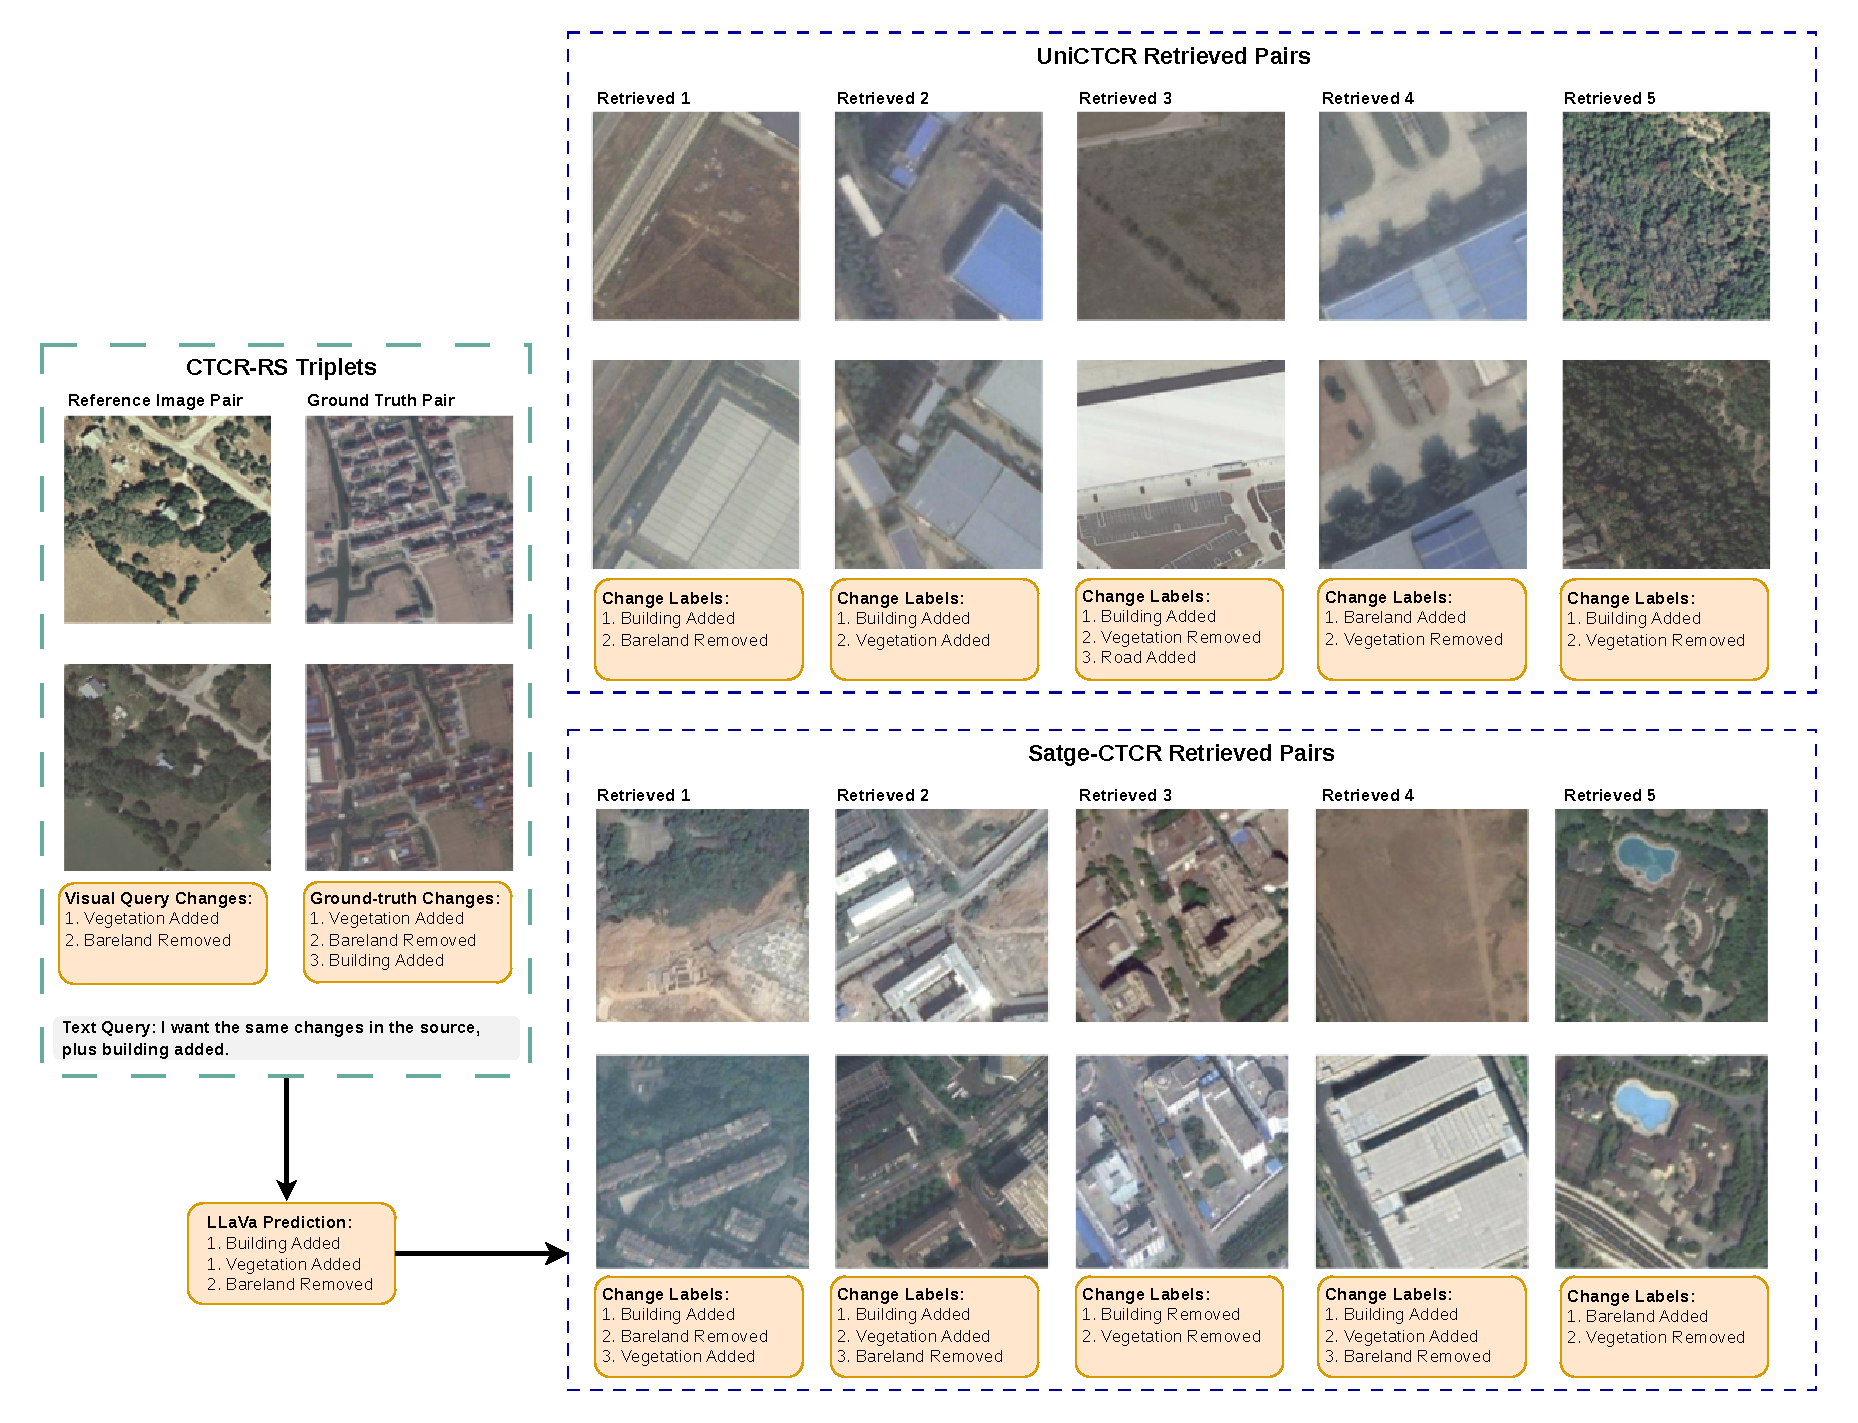
\includegraphics[width=0.85\textwidth]{images/CTCR-RS/supp-figure4.pdf}
    \caption{Qualitative retrieval successes. Given a
    reference pair with 2 visual changes (Vegetation Added,
    Bareland Removed) and a text query (Building Added),
    StageCTCR retrieves 3 correct pairs in the top 5 (ranks
    1, 2, 4), while UniCTCR retrieves pairs that omit
    specific changes. LLaVA-NeXT correctly predicts the full
    change set.}
    \label{fig:chap6_qual_success}
\end{figure}
 
\begin{figure}[ht]
    \centering
    % NOTE: insert Figure 5 from the supplementary here
    % (qualitative retrieval with LLaVA failure: 3 visual
    % changes + 1 text, LLaVA misses Vegetation Removed)
    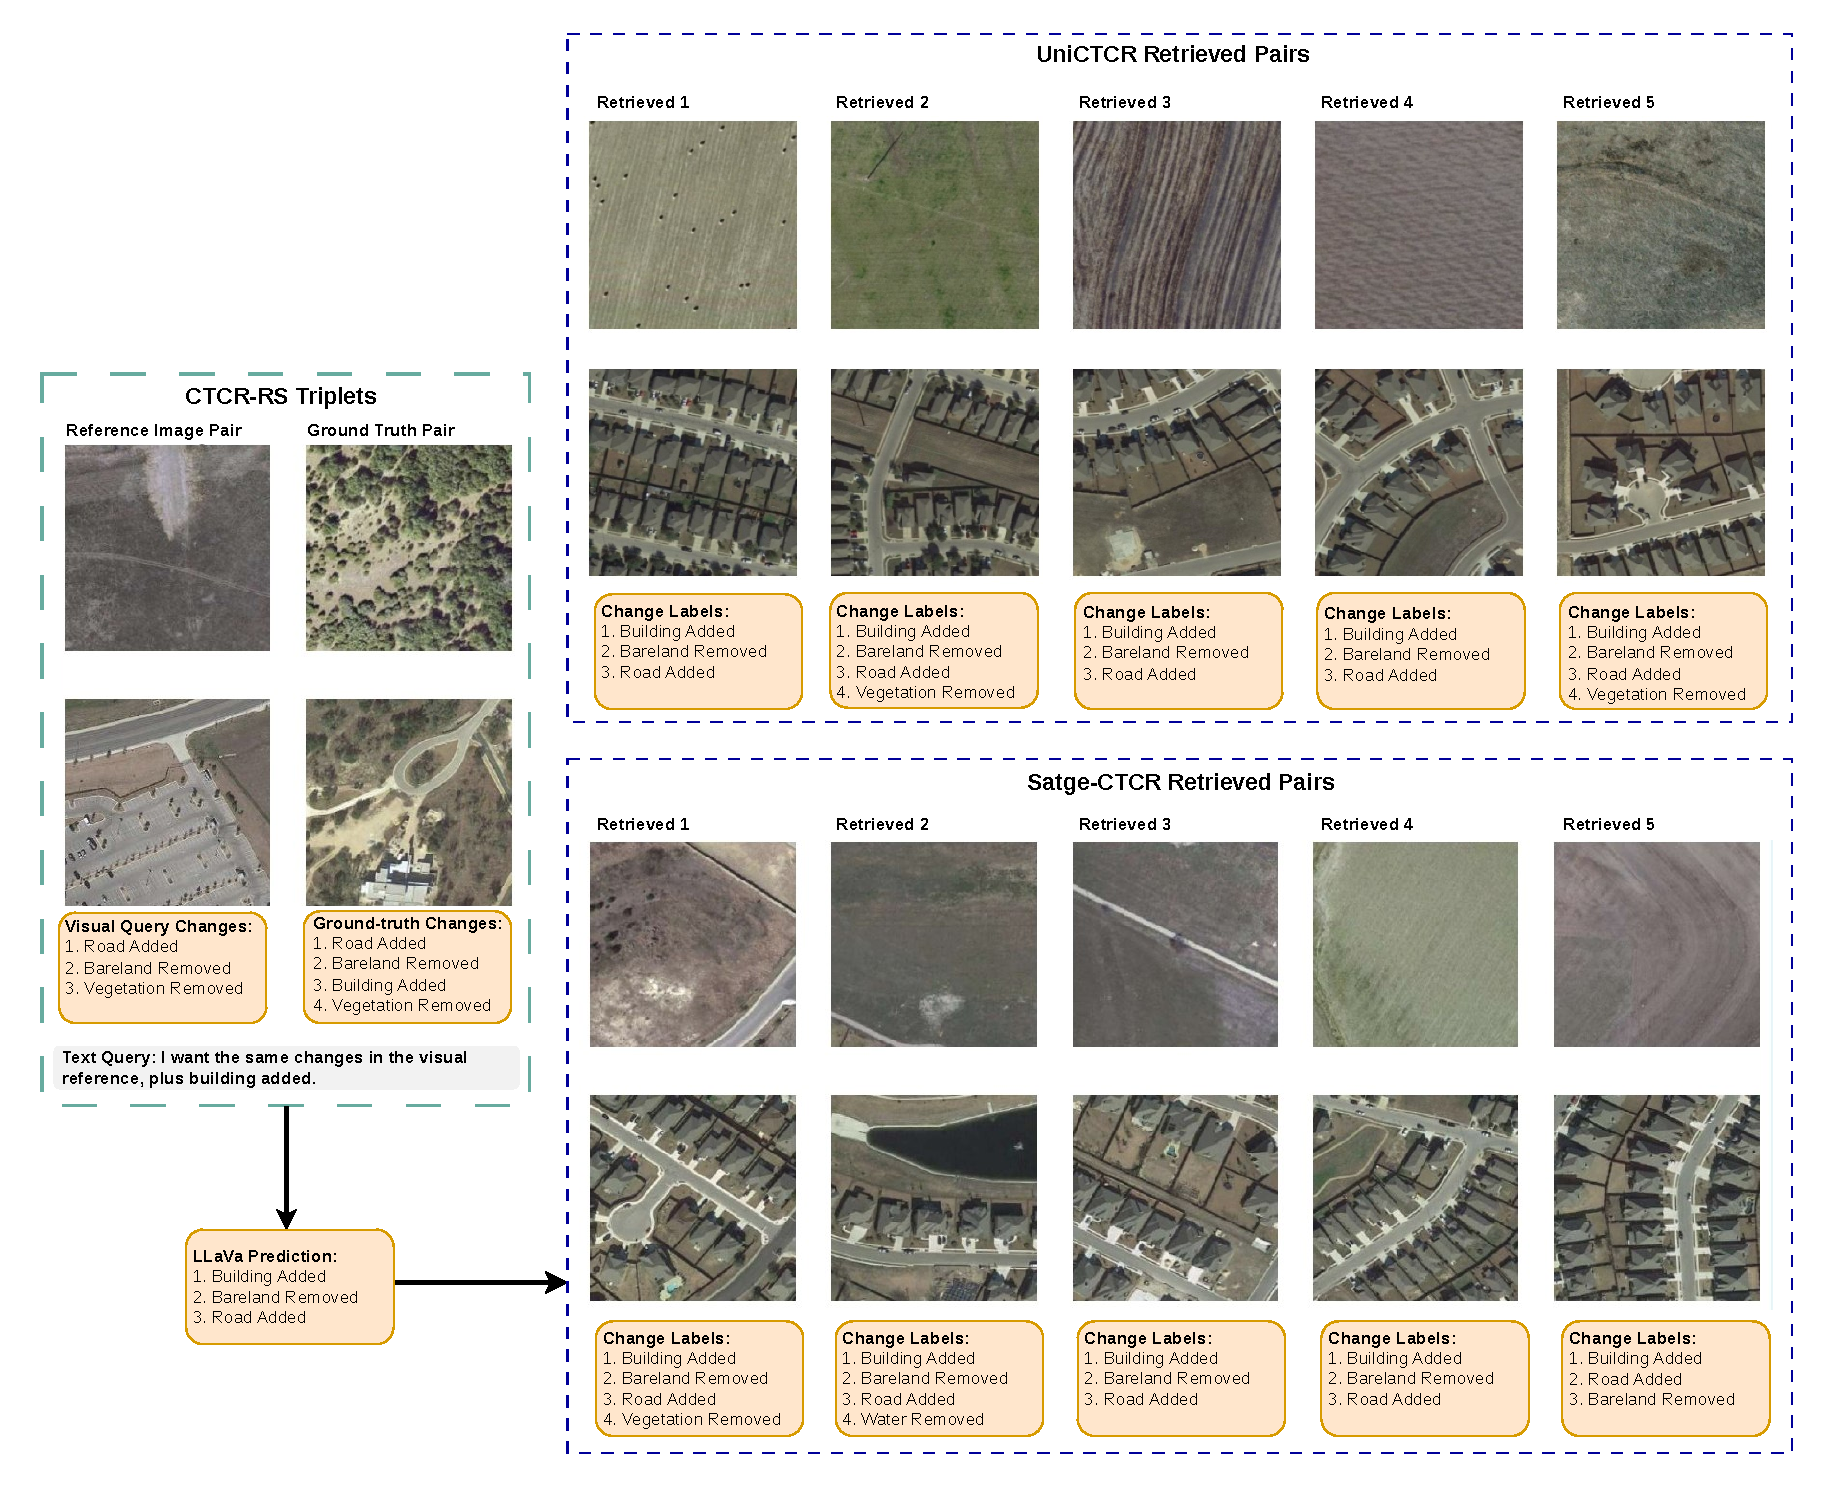
\includegraphics[width=0.85\textwidth]{images/CTCR-RS/supp-figure6.pdf}
    \caption{Impact of Stage~1 composition errors on
    retrieval. Given a reference pair with 3 visual changes
    (Road Added, Bareland Removed, Vegetation Removed) and
    a text query (Building Added), LLaVA-NeXT misses
    Vegetation Removed in its prediction. While the first
    retrieved pair is still correct (likely due to strong
    visual similarity), subsequent results lack the
    Vegetation Removed attribute.}
    \label{fig:chap6_qual_failure}
\end{figure}
 
Figure~\ref{fig:chap6_qual_success} illustrates a success
case in which StageCTCR outperforms UniCTCR due to its
explicit compositional reasoning. Figure~\ref{fig:chap6_qual_failure}
illustrates the cascading failure mode of StageCTCR: a
single missed label in Stage~1 propagates to Stage~2,
where retrieval is steered toward a slightly incorrect
semantic cluster. Despite this, the first retrieved result
is still correct, likely because of strong overall visual
similarity between matching image pairs.
 
% ============================================================
\section{Broader Impact and Ethical Considerations}
\label{sec:chap6_impact}
% ============================================================
 
\subsection{Operational Value}
\label{sec:chap6_impact_value}
 
The CTCR-RS task addresses a genuine bottleneck in
operational Earth Observation workflows. Analysts monitoring
large archives currently face an inhomogeneous query
problem: they may observe a change of interest in one
location and wish to retrieve analogous locations elsewhere
in the archive, but lack the means to specify the composed
visual-textual query efficiently. Existing text-only
retrieval requires exhaustively describing all expected
changes from scratch, a burden that grows with scene
complexity and is particularly acute for concurrent
multi-class transitions (e.g., simultaneous vegetation
removal, building construction, and road addition). The
CTCR-RS formulation reduces this burden: the reference
pair encodes the observed changes implicitly, and the
analyst needs only to specify what is additionally sought.
 
In the long term, a general-purpose CTCR-RS system could
enable applications currently infeasible at scale:
identifying all locations in a global Sentinel-2 archive
where urban expansion has co-occurred with deforestation,
surfacing candidate areas where infrastructure damage has
occurred alongside flooding during disaster response, or
tracking the spread of a specific land-cover transition
pattern across a continent over time. The current work
establishes that the task is tractable and identifies the
key technical bottlenecks; realizing this potential
requires scaling the dataset beyond the urban domain and
developing encoders capable of disentangling dense
multi-class change signatures.
 
\subsection{Dual-Use Risks}
\label{sec:chap6_impact_risks}
 
Retrieval systems capable of identifying specific land-cover
changes at scale are not without risk. The same capability
that accelerates environmental monitoring can, if misused,
enable unauthorized surveillance of sensitive
infrastructure, including military installations or
undisclosed construction activities, raising legitimate
geopolitical concerns that responsible deployment must
account for. The public availability of high-resolution EO
data (Sentinel-1/2, commercial providers) already presents
similar dual-use challenges, but a retrieval system that
can efficiently surface specific change patterns across
global archives amplifies this risk by reducing the
expertise and time required to locate areas of interest.
 
\subsection{Geographic Bias}
\label{sec:chap6_impact_bias}
 
The CTCR-RS dataset inherits the geographic biases of its
source datasets, LEVIR-CC and SECOND-CC, which predominantly
reflect developed urban environments with change patterns
characteristic of rapid urbanization in China and the
United States. As a result, the trained models may
underperform on landscape changes more common in other
regions of the world, including smallholder agricultural
expansion, informal urbanization, or primary deforestation
in the Global South. Additionally, the dataset's strong
concentration of Building Added and Bareland Removed
co-occurrences reflects a specific urbanization dynamic
that is not representative of all geographic contexts.
Prioritizing geographically diverse training distributions
and extending the curation pipeline to datasets covering
more diverse change types and regions is a critical
direction to ensure that performance gains in EO retrieval
translate equitably across global geographies.
 
% ============================================================
\section{Conclusion and Limitations}
\label{sec:chap6_conclusion}
% ============================================================
 
This chapter introduced Composed Temporal Change Retrieval
in Remote Sensing (CTCR-RS), a novel retrieval task that
enables querying EO archives through a combination of
bi-temporal reference image pairs and natural language
instructions specifying additional changes. To support this
task, the CTCR-RS dataset was constructed by normalizing
free-form change captions into a structured 14-class
geospatial ontology, yielding 30,179 compositional triplets
from two established change captioning datasets. Two
baseline architectures were proposed: UniCTCR, which
addresses the task through end-to-end latent fusion, and
StageCTCR, which decomposes the problem into explicit
semantic composition (LLaVA-NeXT via LoRA) followed by
domain-adapted retrieval (CLIP via LoRA). Results
confirm that explicit staged decomposition consistently
outperforms implicit latent fusion, with StageCTCR
surpassing UniCTCR's oracle at inference time.
 
\textbf{Limitations and Perspectives.}
Several limitations should be acknowledged.
First, the dataset is currently scoped to urban land-cover
changes derived from LEVIR-CC and SECOND-CC, limiting
the diversity of geographic contexts, change types, and
scene complexities. Extending the pipeline to multi-domain
datasets covering rural, coastal, and disaster-related
changes is the most important direction for future work.
Second, the textual queries use a fixed template (``I want
the same changes as in the reference pair, plus
[label(s)]''), which provides precision and consistency
but does not reflect the unconstrained, natural language
instructions that analysts would use in practice. Handling
free-form natural language modification queries is an
important open challenge.
Third, global vision encoders produce entangled embeddings
when four or more concurrent changes co-occur in a target
pair, causing performance to degrade severely at $>$2
visual changes. Patch-level or change-specific encoding
strategies are needed to address this limitation.
Fourth, Stage~1 composition errors cascade into Stage~2
retrieval with no mechanism for recovery. A unified model
that can jointly reason about composition and retrieval,
or an uncertainty-aware Stage~2 that discounts
low-confidence Stage~1 predictions, could mitigate this.
Fifth, the dataset construction relies on LLM extraction
with 83.5\% accuracy; the remaining 16.5\% of labels
introduce noise that is difficult to fully eliminate
without exhaustive manual annotation.
 
 